\section{Results}
\label{sec:results}
In this section, we will show and discuss some of the results of the research described in the earlier sections. More specifically: we show how exactly the popularity of various topics changed over time. Since we have a thousand topics, we cannot show charts for every individual topic. Instead, we hand-picked a few topics we consider to be interesting and show these. 

\subsection{Popularity plots}
Note that, since there are 1,000 topics, the average popularity is 0.1\%. The popularity is positively skewed, however: roughly a third of the month/topic combinations have a popularity below one basis point (0.01\%). To stress this point we include figure~\ref{fig:popularitydistribution}, which shows the distribution of monthly popularity from 0.0\% to 1.0\% in steps of 0.1\%.

\begin{figure}[H]
	\caption{Popularity distribution - distribution of popularity (in percent) per month/topic combination}
	\label{fig:popularitydistribution}
	\centering
	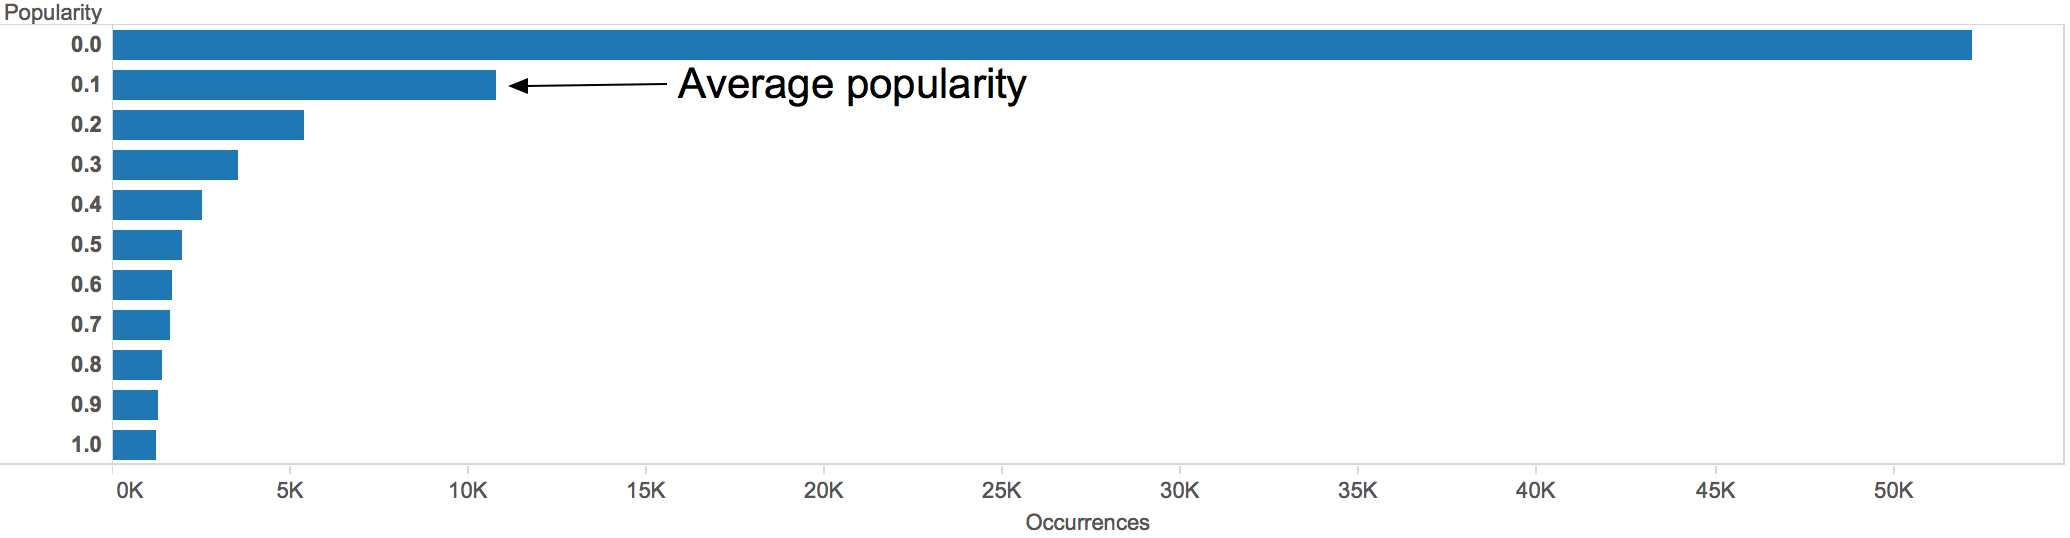
\includegraphics[width=14cm]{popularity_distribution}
\end{figure}

The first chart shows the popularity of the topic with Steve Jobs. As stated before, the news article about his death was the most upvoted article in Hacker News history. As such, one might expect a spike around the time of his death (October 5, 2011). Figure~\ref{fig:trend_jobs} shows one enormous spike, which matches our expectations perfectly.

Steve Wozniak (Jobs' cofounder) is also in this topic, but stayed too much in the background to cause big spikes.
\begin{figure}[H] % Topic 579
	\caption{Popularity of Apple founders Steve Jobs and Wozniak}
	\label{fig:trend_jobs}
	\centering
	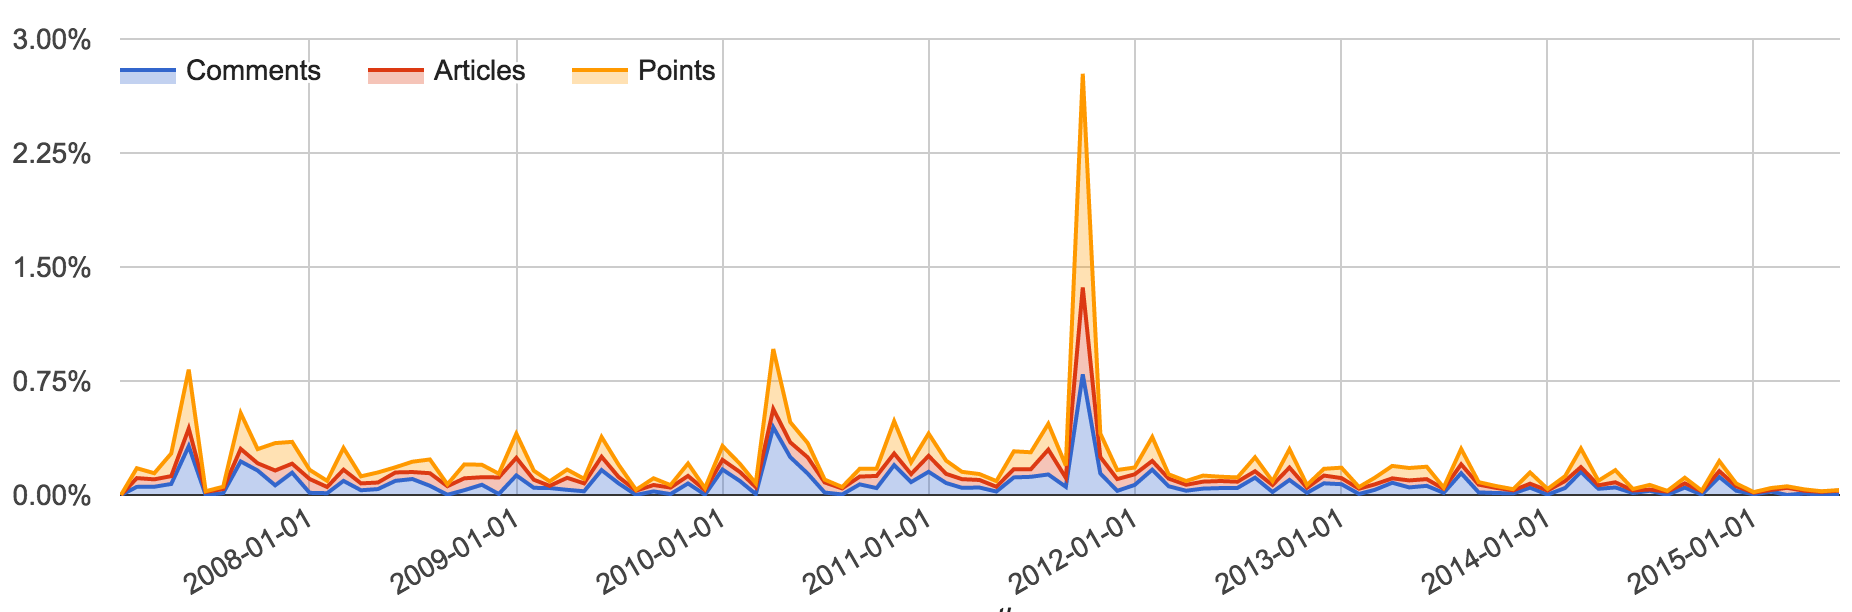
\includegraphics[width=14cm]{topic_trends/jobs_relative}
	% jobs wozniak woz jobs. steve steves jobs's jobssteve imagineers wozs
	% Interesting: Tim Cook is not in this cluster, and his coming out is therefore not visible in this graph
\end{figure}

Another big event in the computer science community was the identification of Edward Snowden. The identity of the famous NSA whistleblower was revealed by the Guardian at June 9, 2013. As with Steve Jobs, we see a huge spike in the popularity of this topic for the same month.

Earlier (small) peaks are caused by other usages of the word whistleblower and/or Wikileaks. After his public identification, he gave a few more interviews which attracted some attention and explain the sustained popularity.
\begin{figure}[H] % Topic 70
	\caption{Popularity of Edward Snowden, Whistleblower, leaks, Reddit}
	\label{fig:trend_snowden}
	\centering
	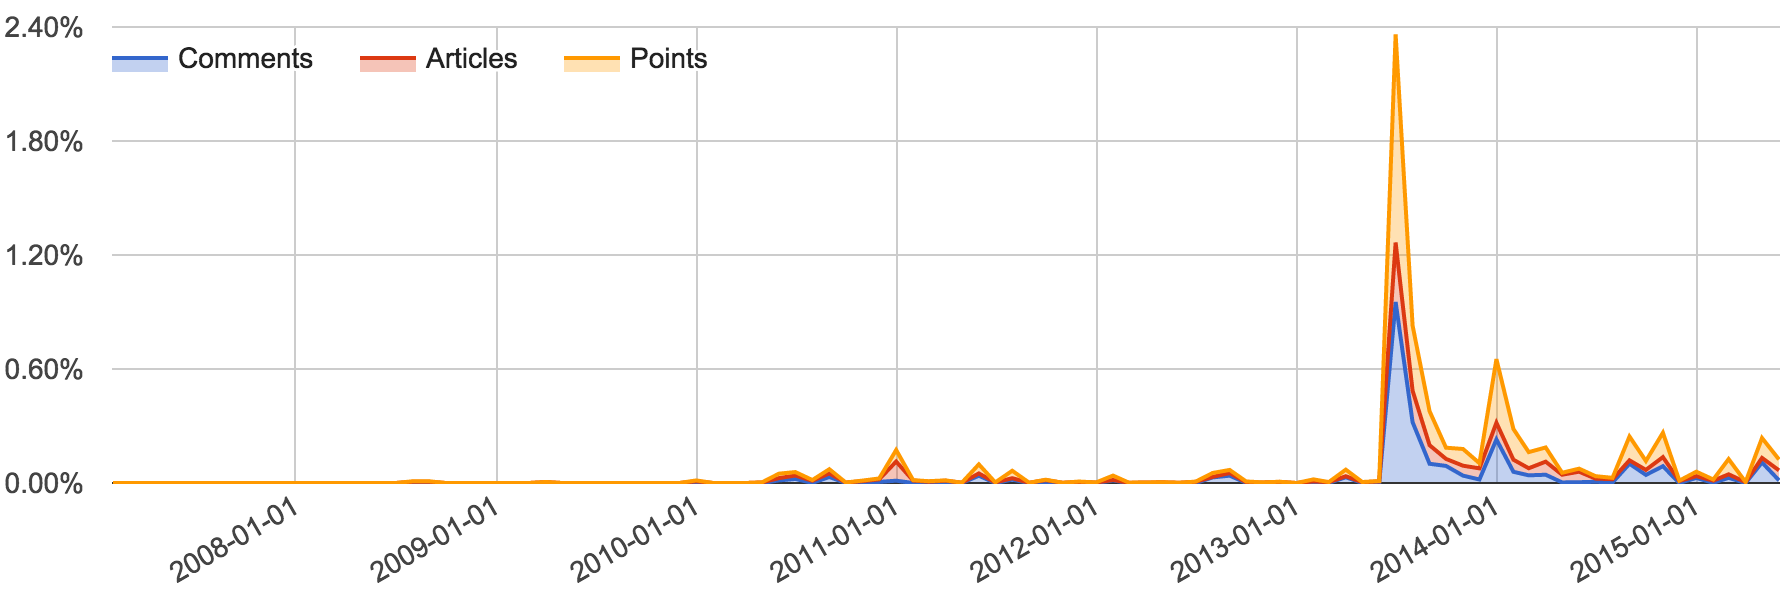
\includegraphics[width=14cm]{topic_trends/snowden_relative}
	% edward whistleblower contractor-turned-whistleblower snowden.the snowden's leaker snowdens reddit.com submitted snowden. snowden.in
\end{figure}

Elon Musk is described by Wired.com as a ''maverick entrepreneur" due to his big and risky projects. We see this reflected in the chart of his popularity (figure~\ref{fig:trend_elon}). Halfway 2010, Elon was out of cash (despite a 200 million dollar buyout from PayPal), which sparked some curiousity. The big spike late 2012 marks his expressed intent to have SpaceX (his spacecraft company) fly to Mars. The biggest spike in the chart, halfway 2013, marks the introduction of Hyperloop, a project for high-speed transportation, owned by Musk.
\begin{figure}[H] % Topic 383
	\caption{Popularity of Elon Musk, SpaceX, Tesla, Hyperloop}
	\label{fig:trend_elon}
	\centering
	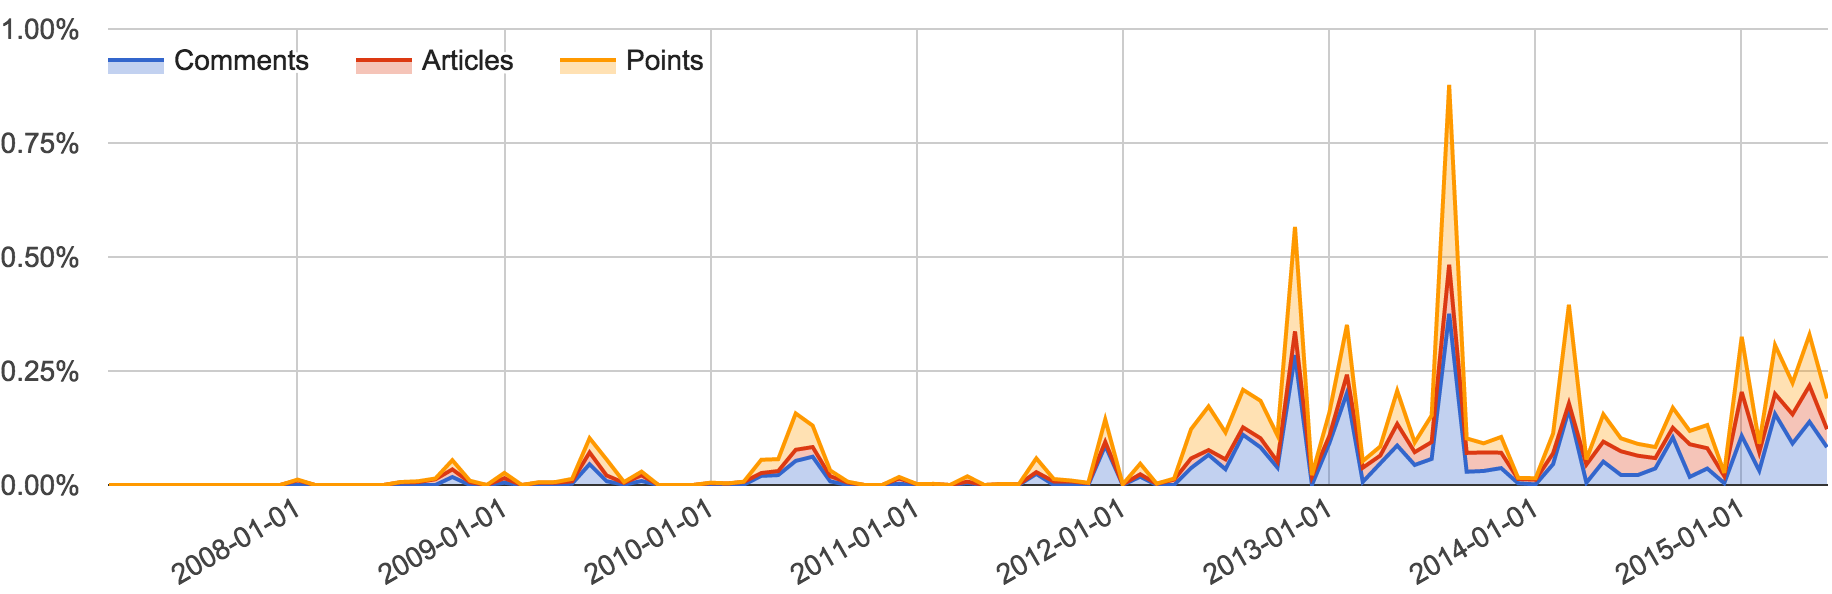
\includegraphics[width=14cm]{topic_trends/elon_relative}
	% elon musks spacex musk's tesla hyperloop test track musk
\end{figure}

\pagebreak
In the popularity charts of keynote-related topics (figure~\ref{fig:trend_keynote}), one can see yearly patterns of spiking popularity. Each June has a spike of over 0.1\%, which corresponds to Apple's annual WWDC (Worldwide Developers Conference). The spikes smaller than 0.1\% are just noise.
\begin{figure}[H] % Topic 79
	\caption{Popularity of keynote, Apple, @scale, developers conference}
	\label{fig:trend_keynote}
	\centering
	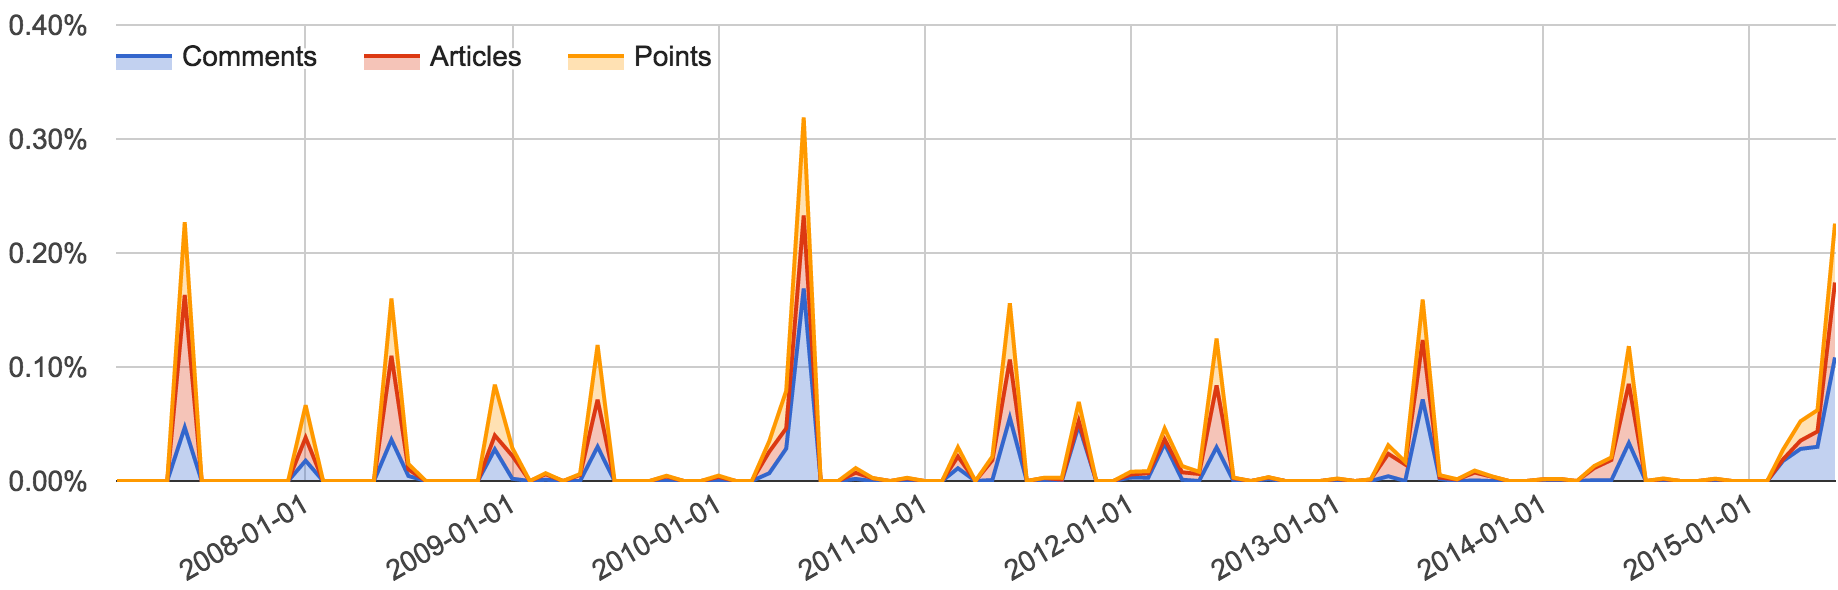
\includegraphics[width=14cm]{topic_trends/keynote_relative}
	% keynote apple live yesterday's apple's @scale apple developers conference keynotes conference macworld
\end{figure}


The next chart (figure~\ref{fig:trend_docker}) shows the increasing popularity of a new and upcoming technique: containerization. Before the releases Docker (2013) and CoreOS (2014) and before that, containerization was already used as a term for seperating Linux processes (which explains earlier peaks). The chart show how the release of Docker 1.0 (June 2014) created a lot of buzz, and the sustained popularity afterwards.

Interestingly, the initial release of Docker did not receive much attention. We think this is because the usecases were a bit vague and the software was not production-ready.
\begin{figure}[H] % Topic 412
	\caption{Popularity of Docker, CoreOS, etcd, containers, OpenStack}
	\label{fig:trend_docker}
	\centering
	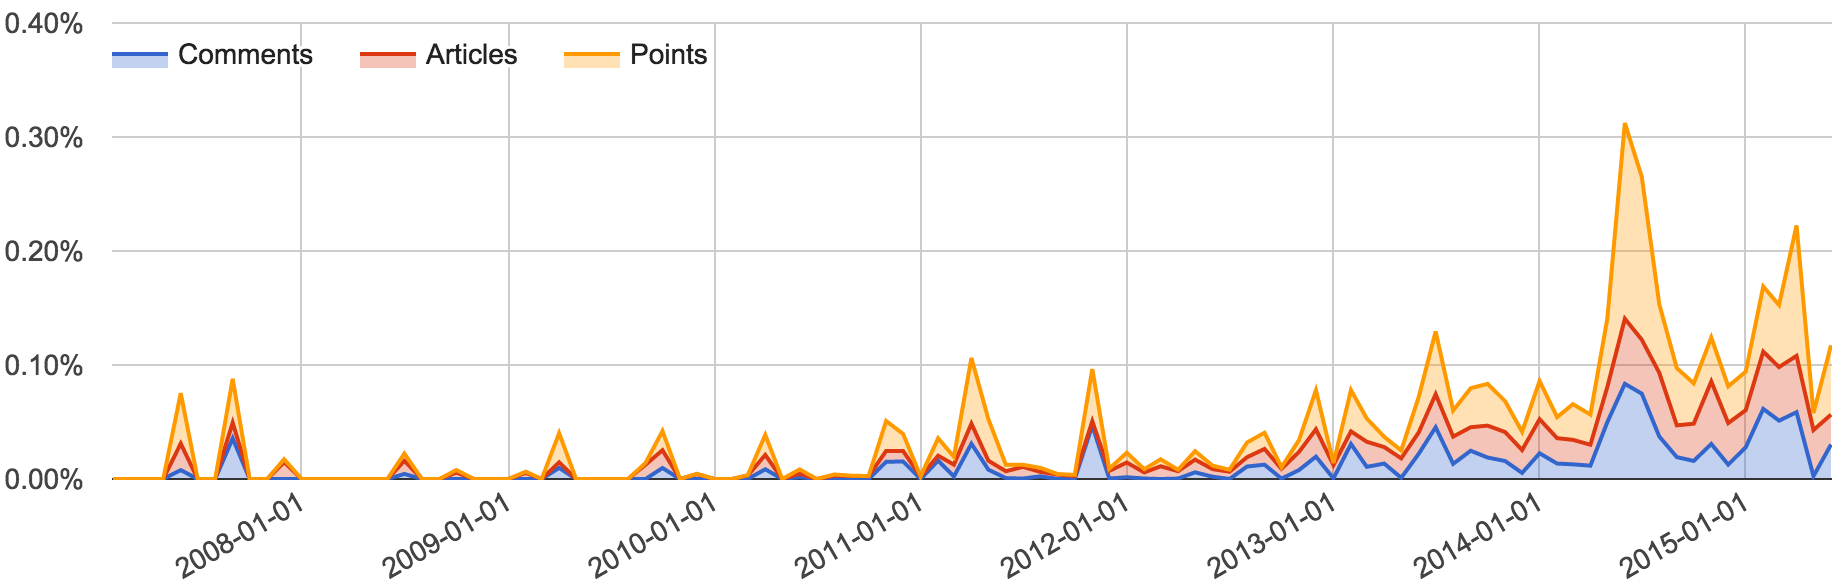
\includegraphics[width=14cm]{topic_trends/docker_relative}
	% docker coreos etcd images:containers openshift mesos deis openstack orchestration dokku
\end{figure}

In the last chart we provide here (figure~\ref{fig:trend_raspberry}), we added two red arrows. These point at the release dates of the Raspberry Pi (version 1 and 2). Before the first release, we already see a growing attention. Since the Raspberry Pi is a crowd-funded project, its creaters already promoted it before the release.
\begin{figure}[H] % Topic 17
	\caption{Popularity of Raspberry Pi, Kindleberry}
	\label{fig:trend_raspberry}
	\centering
	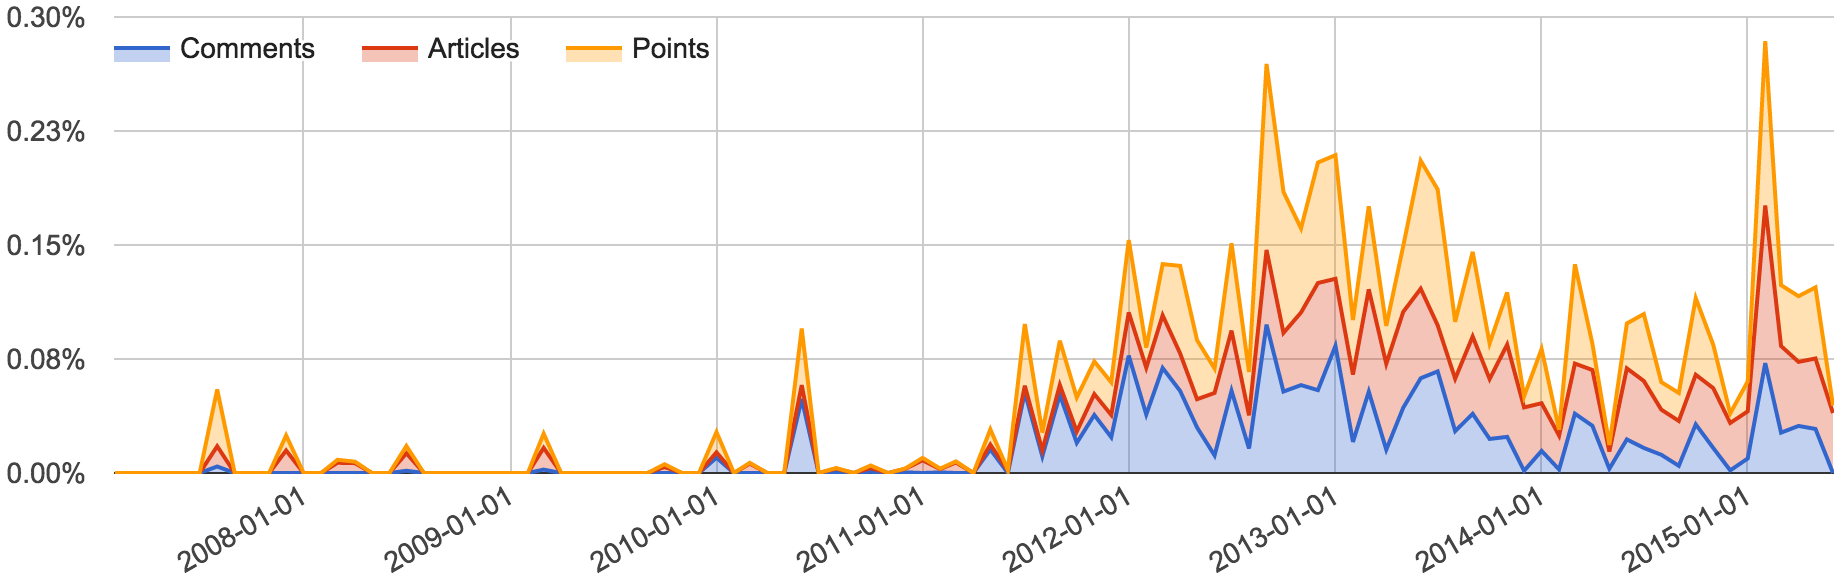
\includegraphics[width=14cm]{topic_trends/raspberry_relative}
	% raspberry pi's kindleberry pis navio+ motherbone-tm-pione-tm- piface razberry rpi raspberrypi
\end{figure}
